\documentclass[12pt]{article}

\usepackage{graphicx}
\graphicspath{{./figures/}}

\usepackage{caption}
\usepackage[font=scriptsize]{subcaption}
\captionsetup[figure]{labelsep=none}
\captionsetup[table]{labelsep=none}
\usepackage{amssymb}
\usepackage{bbm}
\usepackage{amsmath}
\usepackage{import}
\usepackage{array}
\usepackage{enumitem}
\usepackage{booktabs}
\usepackage{indentfirst}
\usepackage{afterpage}
\usepackage{floatrow}
\usepackage{pdflscape}
\usepackage{soul}
\usepackage{float}
\usepackage{adjustbox}
\usepackage{longtable}
\usepackage{setspace}
\usepackage[margin=1in]{geometry}
\usepackage[round]{natbib}
\usepackage{hyperref}
\usepackage{titlesec}
\usepackage{threeparttable}
\usepackage{rotating}
\usepackage{ragged2e}
\usepackage{authblk}

\floatstyle{plaintop}
\restylefloat{table}


\begin{document}

\begin{center}
    {\normalsize \textbf{Disparities in neonatal mortality in India are driven by private, not public facility births}} \\[0.5em]
    {\normalsize \today}
\end{center}



%=====================================================================
% INTRODUCTION
%=====================================================================

\section{Introduction}

Neonatal mortality is an important indicator of the health of a population. The frequency of deaths in the first month of life reflects risks accumulated during pregnancy, the quality of care during and after childbirth, and the long term health of children that survive into adulthood. Social disparities in neonatal mortality are therefore an important indicator for how inequalities in population health may stem from the very beginning of life.

In India, caste and religion are important dimensions of inequalities in health. In this paper, we distinguish five major social groups based on constitutional categories: Adivasi (Scheduled Tribe), Dalit (Scheduled Caste), Other Backward Class (OBCs), Muslim, and forward caste Hindu. Mortality disparities across these social groups are well documented (CITE). However, for neonatal mortality, less is known about whether these disparities are equally large across the different healthcare settings in which births occur. 

This distinction is especially important in India, which has a large system of rural public health facilities alongside a growing private sector where the quality of care varies substantially across regions. We highlight Uttar Pradesh and Bihar in our analysis, two large northern states that comprise over a quarter of India's population together. Neonatal mortality is much higher in Uttar Pradesh and Bihar across every social group, with rates roughly 15 to 20 deaths per 1,000 births above those observed in the rest of India, and is particularly high among rural private sector births. 

Our primary contribution is showing that disparities in neonatal mortality are much wider among private facility births than public facility births in Uttar Pradesh and Bihar. The contrast is especially stark for births to Dalits mothers in these two states: the neonatal mortality gap between Dalit and forward caste births is about 4 deaths per 1,000 in public facilities and 35 deaths per 1,000 in private facilities. In contrast, in other Indian states, the disparity in neonatal mortality between Dalit and forward caste births in private facilities is less than half as large.

Previous research has documented higher neonatal mortality among private than public facility births in poorer north Indian states (\cite{franz2025cheaper, coffey2025excess}). This work points to differences in the quality of care provided as one possible explanation, including incentives facing private providers to offer additional services and newborn care practices that may increase mortality risk, such as early bathing of newborns. Our results add an important dimension to this phenomenon: whatever produces the excess neonatal mortality observed in private facilities does not affect all social groups equally.


We test whether wider disparities in neonatal mortality among private facility births could reflect differential selection into private care. Private facility births among disadvantaged social groups may involve higher underlying risk relative to their public facility births than is the case among Forward Hindus. Thus we compare maternal and birth risk factors, pregnancy and delivery complications, and socioeconomic characteristics between private and public facility births within each social group. Adjusting for these characteristics in regression analysis does little to explain the pattern of larger mortality disparities in private facilities -- in Uttar Pradesh and Bihar, the excess private facility mortality gap for Dalits relative to Forward Hindus remains about 30 deaths per 1,000 even after controlling for observed risk factors and socioeconomic characteristics.

This remaining disparity could arise for at least two other reasons: disadvantaged social groups may give birth in different, lower quality private facilities, or they may receive worse care within the same private facilities. We begin to test the first possibility by adjusting for sampling cluster fixed effects, which compare births in the same local area, and find that the extent to which disadvantaged social groups in Uttar Pradesh and Bihar have larger private–public gaps in neonatal mortality changes little. This suggests that the result is not driven simply by Dalit mothers living in areas served by worse private facilities. We cannot distinguish, however, between the possibility that disadvantaged social groups may sort into lower quality private facilities within the same local area and the possibility that they may get worse care within the same facilities, because the NFHS does not identify the specific facility in which a birth occurred. 

This paper contributes to several areas of the demography literature. First, it contributes to research on social disparities in early life mortality by showing that these disparities vary substantially across the healthcare settings in which births occur. This distinction is important as giving birth in health facilities as opposed to at home is becoming increasingly universal in India and other low and middle income countries. Inequality in early life mortality may depend not only on access to a health facility for birth but also the type and quality of health facility being chosen. 

Second, the paper contributes to research on the role of the private health sector in maternal and child health. We show that general differences between birth outcomes in public and private health facilities conceal important inequalities across social groups. As the private healthcare sector grows in India and other low and middle income countries, it will be important to study the consequences on population health, as well as how they are distributed across social groups. 


\section{Data}

We use the birth recode from the fourth and fifth rounds of India’s National Family Health Survey (NFHS), conducted in 2015–16 and 2019–21. The NFHS is India’s Demographic and Health Surveys (DHS) and is publicly available at \textit{dhsprogram.com}. The survey uses a two-stage clustered sampling design and collects complete birth histories from women ages 15–49. Our analysis focuses on births occurring in the five years preceding each survey to mothers residing in rural areas. Neonatal mortality is defined as deaths within the first 28 days of life.

\section{Variables}

To investigate possible explanations for the larger excess mortality observed among private facility births to disadvantaged social groups, we examine a set of maternal and birth risk factors. These include whether the mother was younger than 20 at the time of birth, projected maternal underweight at the beginning of pregnancy (FOOTNOTE), mode of delivery, child sex, multiple birth, prior neonatal death, and birth order (\cite{coffey2025excess}, CITE). For the most recent birth, the NFHS also asks about complications during pregnancy and delivery, including breech presentation, prolonged labor, and excessive bleeding, as well as newborn care practices such as initiation of breastfeeding within one hour and skin-to-skin contact. We use these variables to understand whether births in private facilities have higher underlying risk.

An important risk factor for neonatal death is if the mother is underweight at the start of pregnancy. Using this, we estimate the BMI of women before their most recent pregnancy if they are not pregnant, or before their current pregnancy if they are pregnant at the time of the survey.
 
We first estimate the relationship between BMI and age among nonpregnant women in each state and use this relationship to adjust each woman’s BMI at the time of the survey to the age at which she began her most recent or current pregnancy. We then estimate the relationship between BMI and gestational duration among pregnant women in each state and use this relationship to adjust each pregnant woman's BMI at the time of the survey to the first trimester. We classify women as projected to have been underweight before pregnancy if their estimated prepregnancy BMI is below 18.5 kg/m².

We additionally include socioeconomic characteristics, including maternal literacy and household wealth quintile. The DHS wealth index is constructed from information on household assets and housing characteristics and summarizes relative household socioeconomic status within the survey population.

\section{Methods}

To test for differences in the characteristics of births between public and private health facilities, we estimate simple regressions of characteristics associated with neonatal mortality risk on an indicator for private facility birth. We estimate these regressions separately for each social group and region:

\begin{equation}
Y_i = \alpha + \beta Private_i + \varepsilon_i,
\end{equation}

where \(Y_i\) denotes a maternal or birth risk factor, pregnancy or delivery complication, socioeconomic characteristic, or measure of care at birth. The coefficient \(\beta\) therefore captures the difference in the mean of each characteristic between private and public facility births within a given social group and region. Regressions use NFHS sampling weights, and standard errors are clustered at the primary sampling unit level to account for the clustered survey design.

To test whether the pattern of higher neonatal mortality in private facility compared to public facility births is more severe among disadvantaged social groups, we estimate a regression of neonatal mortality on indicators for social group, private facility birth, and the interaction between these two variables.

\begin{equation}
NNM_i = \alpha + \beta_g Group_i + \beta_p Private_i
+ \beta_{gp}(Group_i \times Private_i)
+ X_i'\gamma + \delta_r + \mu_c + \varepsilon_i.
\end{equation}

Here \(NNM_i\) is an indicator for neonatal death for birth \(i\), scaled by 1,000 so that coefficients can be interpreted in deaths per 1,000 births. \(Group_i\) denotes indicators for social group, and \(Private_i\) is an indicator for birth in a private facility. \(X_i\) contains the maternal and birth risk, pregnancy and delivery complication, and socioeconomic characteristics that are predictive of neonatal death risk. \(\delta_r\) denotes survey round fixed effects, and \(\mu_c\) denotes sampling cluster fixed effects.

We estimate three specifications for each region. The first includes social group, private facility birth, their interactions, and survey round fixed effects. The second adds controls for neonatal death risk, \(X_i\). The third adds sampling cluster fixed effects, \(\mu_c\).

In all regressions, standard errors are clustered at the primary sampling unit level and observations are weighted by sample weights in accordance with the two stage random sampling design of the NFHS. 



\section{Results}

Figure \ref{fig:fig1} depicts overall neonatal mortality disparities across social groups in rural India. In both Uttar Pradesh and Bihar and in the rest of India, neonatal mortality among births to Dalit mothers is about 8 deaths per 1,000 higher than among births to Forward Hindu mothers.

Neonatal mortality is also about 9 deaths per 1,000 higher among births to Adivasi mothers than among births to Forward Hindu mothers. This difference is not statistically significant in Uttar Pradesh and Bihar, where the Adivasi sample is relatively small.



In Uttar Pradesh and Bihar, neonatal mortality is also high among Adivasi and Muslim births, although confidence intervals are wide for some comparisons. Outside Uttar Pradesh and Bihar, Adivasi and Dalit births have the highest neonatal mortality rates, with both groups experiencing substantially higher mortality than OBC, Muslim, and Forward Hindu births.


Figure \ref{fig:fig2} depicts overall neonatal mortality disparities across social groups in rural India. In both Uttar Pradesh and Bihar and in the rest of India, neonatal mortality among births to Dalit mothers is about 8 deaths per 1,000 higher than among births to Forward Hindu mothers.

Neonatal mortality is also about 9 deaths per 1,000 higher among births to Adivasi mothers than among births to Forward Hindu mothers. This difference is not statistically significant in Uttar Pradesh and Bihar, where the Adivasi sample is relatively small. Neonatal mortality rates among OBC, Muslim, and Forward Hindu births are otherwise relatively similar within both regions.

%=====================================================================
% FIGURE 1
%=====================================================================

\begin{figure}[H]
    \centering

    \includegraphics[
        width=\textwidth
    ]{figures/figure1 overall nnm UP Bihar other
    states NFHS4,5.png}

    \caption{
        : Disparities in neonatal mortality for all rural births
    }
    \label{fig:fig1}

    \vspace{0.4em}

    \begin{minipage}{0.96\textwidth}
        \scriptsize
        \textit{Notes:}
        The sample consists of rural births in NFHS-4 and NFHS-5.
    \end{minipage}
\end{figure}


Figure \ref{fig:fig2} now separates public and private facility births in depicting disparities in neonatal mortality. Among public facility births in Uttar Pradesh and Bihar, neonatal mortality rates are relatively similar across social groups, ranging from about 32 to 38 deaths per 1,000 births. In contrast, disparities are much larger among private facility births. The contrast is especially stark for births to Dalit mothers in Uttar Pradesh and Bihar: the difference in neonatal mortality with births to forward caste Hindu mothers is about 35 deaths per 1,000 among private facility births. 


Among private facility births in other Indian states, this difference is also present, albeit less drastically -- neonatal mortality among births to Dalit mothers is 15 deahts per 1,000 births higher than among births to forward caste Hindu mothers, which is half the size of the corresponding gap in Uttar Pradesh and Bihar. 




\begin{figure}[H]
    \centering

    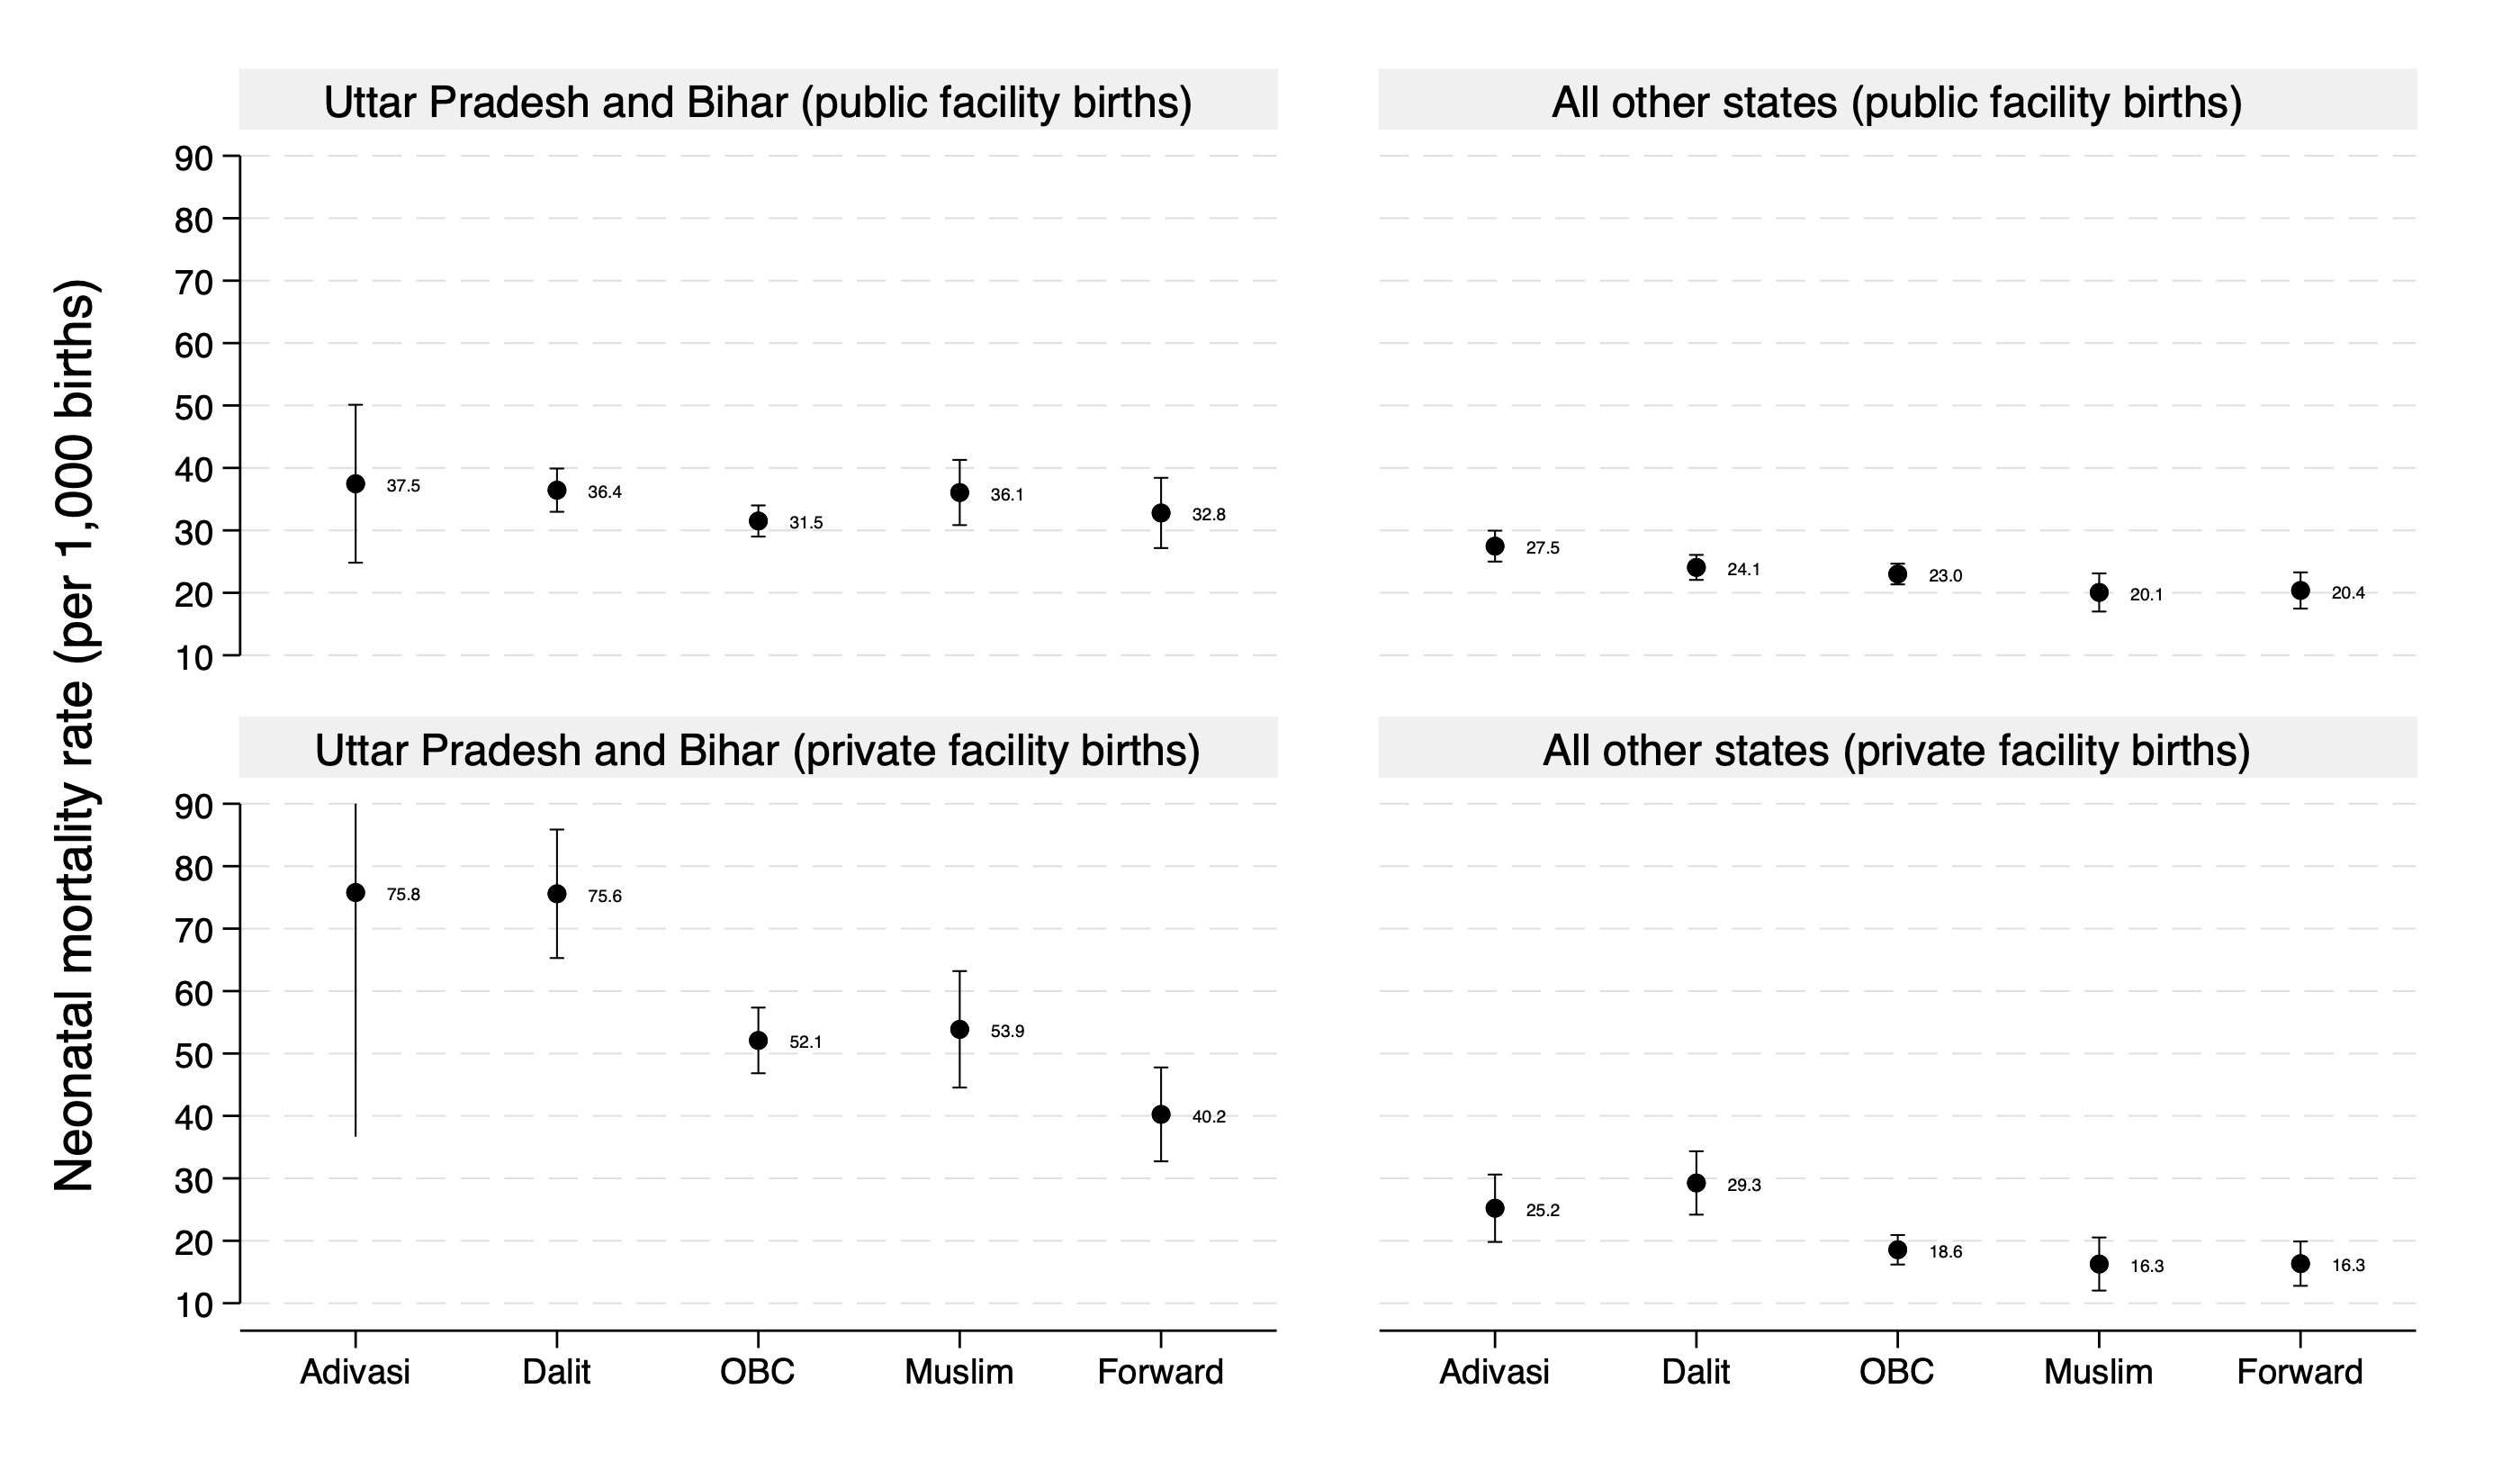
\includegraphics[
        width=\textwidth
    ]{figures/figure2 nnm public private UP Bihar NFHS4,5.png}

    \caption{
        : Disparities in neonatal mortality for rural births by facility type
    }
    \label{fig:fig2}

    \vspace{0.4em}

    \begin{minipage}{0.96\textwidth}
        \scriptsize
        \textit{Notes:}
        The sample consists of rural births in NFHS-4 and NFHS-5.
    \end{minipage}
\end{figure}


Table \ref{tab:private_public_characteristics} begins to test whether there are differences between private and public facilities in characteristics that may explain the differences in neonatal mortality. 

Several characteristics show meaningful differences -- among all social groups, women who give birth in private facilities are up to 10.8 percentage points less likely to have been underweight at the start of pregnancy than those who give birth in public facilities. 

%=====================================================================
% TABLE 1
%=====================================================================


\begin{landscape}

\renewcommand{\arraystretch}{1.4}
\setlength{\tabcolsep}{9pt}

\begin{table}[H]
    \centering
    \caption{
        : Differences between private and public facility births by social group and region
    }
    \label{tab:private_public_characteristics}

    \vspace{0.4em}

    \begin{threeparttable}

        \footnotesize

        \begin{adjustbox}{max width=\linewidth}
        \scriptsize
            \begin{tabular}{l*{5}{c}@{\hspace{1.4em}}c@{\hspace{1.4em}}*{5}{c}}
\toprule
& \multicolumn{5}{c}{Uttar Pradesh and Bihar} & & \multicolumn{5}{c}{All other states} \\
\cmidrule(lr){2-6} \cmidrule(lr){8-12}
\addlinespace[0.25em]
& \tiny Adivasi & \tiny Dalit & \tiny OBC & \tiny Forward & \tiny Muslim & & \tiny Adivasi & \tiny Dalit & \tiny OBC & \tiny Forward & \tiny Muslim \\
\midrule
&&&&&&&&&&&\\
\textbf{Maternal and birth risk}&&&&&&&&&&&\\
\hspace*{2em}Mother under 20 at birth&-1.2&-0.5&0.3&-0.8&0.1&&1.0&-1.9***&-0.8*&-2.6***&-4.3***\\
\hspace*{2em}Male child&6.0*&2.1**&3.4***&3.1**&0.7&&2.4**&1.1&0.4&0.6&0.9\\
\hspace*{2em}Multiple birth&2.5&1.8***&1.3***&1.0*&1.2**&&0.6&1.5***&1.7***&1.3***&1.1**\\
\hspace*{2em}Prior neonatal death to mother&3.3*&2.0***&0.8***&0.4&0.2&&0.2&0.9***&0.2&-0.3&-0.1\\
\hspace*{2em}Projected maternal underweight&-10.8***&-8.4***&-7.7***&-8.4***&-9.5***&&-3.8***&-5.1***&-4.8***&-5.7***&-6.1***\\
\hspace*{2em}Birth order&-0.14&-0.34***&-0.34***&-0.37***&-0.39***&&-0.23***&-0.19***&-0.18***&-0.15***&-0.19***\\
&&&&&&&&&&&\\
\textbf{Pregnancy and delivery complications}&&&&&&&&&&&\\
\hspace*{2em}Breech presentation&1.8&1.6**&0.1&-0.4&0.4&&1.4&-0.7&0.9*&0.3&4.4***\\
\hspace*{2em}Prolonged labor&11.9***&7.2***&3.8***&1.7&2.3&&0.6&-4.5***&-3.9***&-2.7***&-4.8***\\
\hspace*{2em}Excessive bleeding&4.6&2.2*&-1.6**&-2.6*&-2.8*&&-2.1&-4.2***&-3.2***&-2.8***&-6.8***\\
\hspace*{2em}C-section birth&25.0***&29.3***&29.7***&34.4***&27.4***&&27.8***&32.0***&31.0***&28.6***&29.6***\\
&&&&&&&&&&&\\
\textbf{Socioeconomic characteristics}&&&&&&&&&&&\\
\hspace*{2em}Mother illiterate&-14.2***&-12.6***&-16.0***&-14.8***&-16.0***&&-18.5***&-9.7***&-10.1***&-9.7***&-13.3***\\
\hspace*{2em}Mean wealth quintile (1--5)&0.54***&0.54***&0.65***&0.73***&0.77***&&0.84***&0.63***&0.69***&0.79***&1.02***\\
&&&&&&&&&&&\\
\textbf{Care at birth}&&&&&&&&&&&\\
\hspace*{2em}Breastfeeding initiated within 1 hour&-3.6&-9.7***&-9.4***&-9.0***&-7.8***&&-8.7***&-7.8***&-7.8***&-7.5***&-1.4\\
\hspace*{2em}Skin-to-skin contact&-11.5**&-21.6***&-21.6***&-25.6***&-18.6***&&-11.5***&-8.1***&-6.2***&-7.9***&-1.8\\
&&&&&&&&&&&\\
\textbf{General}&&&&&&&&&&&\\
\hspace*{2em}Percent births in private facilities&18.1&18.7&24.9&37.6&28.5&&13.3&19.8&31.4&37.0&25.6\\
\hspace*{2em}Sample size&1,604&19,713&36,197&8,576&9,677&&54,587&42,212&66,819&29,223&23,134\\
\bottomrule
\end{tabular}

        \end{adjustbox}

    \end{threeparttable}

    \vspace{0.5em}

    \begin{minipage}{0.92\linewidth}
        \scriptsize
        \textit{Notes:}
        Entries report differences between private and public facility births
        (private minus public) within each social group and region.
        
        
        Each entry is the coefficient on an indicator for private facility birth from a weighted regression of the characteristic in question on private facility birth, with standard errors clustered at the sampling cluster level. Binary characteristics are reported in percentage points. * $p<0.10$, ** $p<0.05$, *** $p<0.01$.
        
        \vspace{0.4em}

        The sample consists of rural public and private facility births in NFHS 4 and NFHS 5. Projected maternal underweight is calculated using the exact same code as the Social Science and Medicine paper. 

    \end{minipage}

\end{table}

\setlength{\tabcolsep}{6pt}
\renewcommand{\arraystretch}{1}

\end{landscape}


%=====================================================================
% TABLE 2
%=====================================================================

\begin{landscape}
    
\renewcommand{\arraystretch}{1.2}
\setlength{\tabcolsep}{12pt}


\begin{table}[H]
    \centering
    \caption{
        : Differences in excess private neonatal mortality across social groups and regions
    }
    \label{tab:nnm_interactions}

    \vspace{0.4em}

    \begin{threeparttable}

        \begin{adjustbox}{max width=\textwidth}
        \scriptsize
            {
\def\sym#1{\ifmmode^{#1}\else\(^{#1}\)\fi}
\begin{tabular}{l*{6}{c}}
\toprule
            &\multicolumn{3}{c}{Uttar Pradesh and Bihar}                      &\multicolumn{3}{c}{All other states}                             \\\cmidrule(lr){2-4}\cmidrule(lr){5-7}
            &\multicolumn{1}{c}{(1)}&\multicolumn{1}{c}{(2)}&\multicolumn{1}{c}{(3)}&\multicolumn{1}{c}{(4)}&\multicolumn{1}{c}{(5)}&\multicolumn{1}{c}{(6)}\\
            &\multicolumn{1}{c}{No controls}&\multicolumn{1}{c}{Risk controls}&\multicolumn{1}{c}{+ Cluster FE}&\multicolumn{1}{c}{No controls}&\multicolumn{1}{c}{Risk controls}&\multicolumn{1}{c}{+ Cluster FE}\\
\midrule
Intercept (Forward public reference)&        25.0\sym{***}&        33.1\sym{***}&        26.6\sym{***}&        13.1\sym{***}&        14.5\sym{***}&        15.5\sym{***}\\
            &       (2.9)         &       (5.0)         &       (5.4)         &       (1.2)         &       (2.0)         &       (2.4)         \\
\addlinespace
Adivasi     &        -3.3         &        -8.3         &         1.7         &         5.7\sym{***}&         1.0         &         0.4         \\
            &       (5.7)         &       (5.7)         &       (6.1)         &       (1.5)         &       (1.6)         &       (2.3)         \\
\addlinespace
Dalit       &         3.1         &        -2.1         &         5.1         &         3.1\sym{**} &         1.2         &         0.9         \\
            &       (3.3)         &       (3.3)         &       (4.1)         &       (1.4)         &       (1.4)         &       (1.9)         \\
\addlinespace
OBC         &        -0.5         &        -3.8         &         3.8         &         2.0         &         1.1         &        -1.5         \\
            &       (3.1)         &       (3.0)         &       (3.7)         &       (1.4)         &       (1.4)         &       (1.8)         \\
\addlinespace
Muslim      &         1.6         &        -3.1         &        -3.5         &         1.7         &        -0.5         &         1.3         \\
            &       (3.7)         &       (3.7)         &       (5.0)         &       (1.9)         &       (1.9)         &       (2.8)         \\
\addlinespace
Private facility&         2.1         &         1.5         &         5.0         &        -3.0\sym{*}  &        -1.1         &        -2.3         \\
            &       (4.4)         &       (4.4)         &       (5.0)         &       (1.7)         &       (1.8)         &       (2.4)         \\
\addlinespace
Adivasi $\times$ Private&        27.1         &        23.1         &        24.0         &         0.3         &         1.2         &         5.8         \\
            &      (17.0)         &      (17.0)         &      (17.9)         &       (3.2)         &       (3.2)         &       (4.1)         \\
\addlinespace
Dalit $\times$ Private&        35.2\sym{***}&        32.1\sym{***}&        29.6\sym{***}&         4.7\sym{*}  &         4.2         &         4.5         \\
            &       (7.0)         &       (6.9)         &       (7.5)         &       (2.8)         &       (2.8)         &       (3.3)         \\
\addlinespace
OBC $\times$ Private&        15.8\sym{***}&        15.0\sym{***}&        10.0\sym{*}  &         0.5         &        -0.1         &         0.3         \\
            &       (5.3)         &       (5.2)         &       (5.9)         &       (2.1)         &       (2.1)         &       (2.7)         \\
\addlinespace
Muslim $\times$ Private&        15.6\sym{**} &        15.8\sym{**} &        11.2         &         1.0         &         2.6         &         1.0         \\
            &       (7.0)         &       (6.9)         &       (8.1)         &       (3.1)         &       (3.1)         &       (4.0)         \\
\midrule
Maternal and birth risk controls&                     &  \checkmark         &  \checkmark         &                     &  \checkmark         &  \checkmark         \\
Pregnancy/delivery complication controls&                     &  \checkmark         &  \checkmark         &                     &  \checkmark         &  \checkmark         \\
Socioeconomic controls&                     &  \checkmark         &  \checkmark         &                     &  \checkmark         &  \checkmark         \\
Survey round FE&  \checkmark         &  \checkmark         &  \checkmark         &  \checkmark         &  \checkmark         &  \checkmark         \\
Cluster FE  &                     &                     &  \checkmark         &                     &                     &  \checkmark         \\
Observations&      54,037         &      52,926         &      52,743         &     169,188         &     166,334         &     164,042         \\
\bottomrule
\end{tabular}
}

        \end{adjustbox}


\begin{minipage}{0.92\textwidth}
\scriptsize
\textit{Notes:}
Each column reports a regression of neonatal mortality on social group, private facility birth, their interaction, and the controls indicated in the table. Maternal and birth risk controls include prior neonatal death, projected maternal prepregnancy underweight, child sex, maternal age under 20, multiple birth, and birth order. Pregnancy and delivery controls include vaginal birth, breech presentation, prolonged labor, and excessive bleeding. Socioeconomic controls include maternal illiteracy and wealth quintile. The sample consists of rural public and private facility births in NFHS 4 and NFHS 5. Regressions use NFHS sampling weights and standard errors clustered by PSU. * $p<0.10$, ** $p<0.05$, *** $p<0.01$.
\end{minipage}


    \end{threeparttable}
\end{table}

\setlength{\tabcolsep}{6pt}
\renewcommand{\arraystretch}{1}


\end{landscape}


\bibliographystyle{apalike}
\bibliography{writing/references}
\end{document}
